\documentclass[12pt, twoside]{article}
\usepackage[letterpaper, margin=1in, headsep=0.5in]{geometry}
\usepackage[english]{babel}
\usepackage[utf8]{inputenc}
\usepackage{amsmath}
\usepackage{amsfonts}
\usepackage{amssymb}
\usepackage{tikz}
\usetikzlibrary{quotes, angles}
\usepackage{graphicx}
\usepackage{enumitem}
\usepackage{multicol}

\newif\ifmeta
\metatrue %print standards and topics tags

\title{Regents Geometry}
\author{Chris Huson}
\date{January 2022}

\usepackage{fancyhdr}
\pagestyle{fancy}
\fancyhf{}
\renewcommand{\headrulewidth}{0pt} % disable the underline of the header
\raggedbottom

\fancyhead[LE]{\thepage}
\fancyhead[RO]{\thepage \\ Name: \hspace{4cm} \,\\}
\fancyhead[LO]{BECA / Dr. Huson / Geometry 6 Trigonometry}

\begin{document}
\subsubsection*{6.14 Pre-Quiz: Tangent applications \hfill CCSS.HSG.SRT.C.8}

\begin{enumerate}
\item The diagram shows a buildomg with student A on the ground waving up to student B. Point A is 19 feet from the base of the building, and the angle of elevation from A to B is $32^\circ$.
 
Find how high up student B is from the groundto the \emph{nearest foot}. \hfill (not drawn to scale)
  \begin{flushright}
    \begin{tikzpicture}[scale=0.4]
      %\draw [-, thick] (0,0)--(35:23);
      \draw [-, thick] (-4,0)--
      (0,0)--
        (17,0)--
        (22,0)--
        (22,10)--(17,10)--(17,0);
      \draw [fill] (0,0) circle [radius=0.1] node[above]{$A$};
      \draw [fill] (17,10) circle [radius=0.1] node[above right]{$B$};
      \draw [dashed] (0,0)--(17,10);
      \node at (3, 0)[above]{$32^\circ$};
      \node at (-3, 0)[above]{ground};
      \node at (19.5, 5)[above]{school};
    \end{tikzpicture}
    \end{flushright}

\item From the top of a subway station, a person is visible at an angle of depression of $21^\circ$. If the subway station is 60 feet tall, determine the distance from the person to the base of the subway station, x, to the \emph{nearest foot}.
\begin{center}
    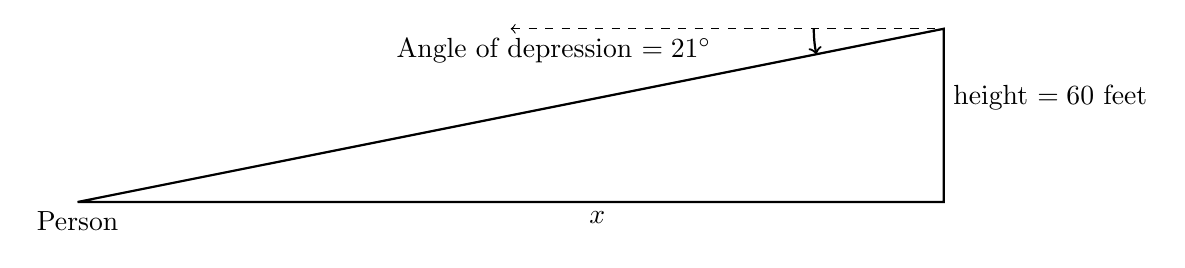
\begin{tikzpicture}[scale=1.1]
      \draw [thick] (10,0)--(0,0)--(10,2.0)--cycle;
      \draw [dashed, <-] (5,2)--(10,2.0);
      \draw [thick, ->] (8.5,2) arc [start angle=180, end angle=191.3, radius=1.5];
      \node at (5.5,2)[below]{Angle of depression $=21^\circ$};
      \node at (10,1.2)[right]{height $=60$ feet};
      \node at (6,0)[below]{$x$};
      \node at (0,0)[below]{Person};
    \end{tikzpicture}
  \end{center} \vspace{2cm}

\item A child sleds from the top of a hill to a group of friends standing at the base of the hill. The hill is 21 feet tall, and the hill's incline is $13^\circ$. Find the distance, d, from the sledder to the group of friends to the \emph{nearest foot}.

(hint: first find the distance to the from the group to the hill horizontally, then use the Pythagorean theorem to find the hypotenuse, d)\\[0.25cm]
  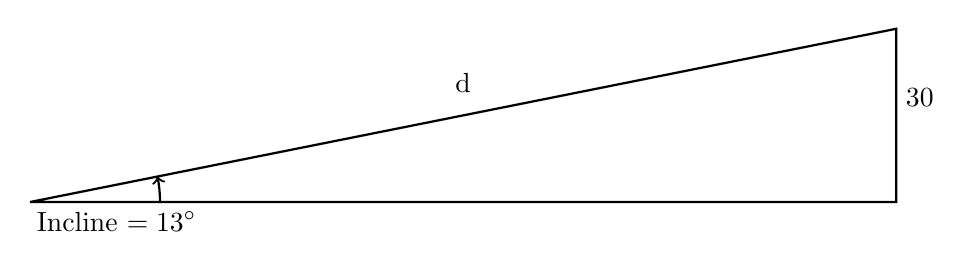
\begin{tikzpicture}[scale=1.1]
    \draw [thick] (10,0)--(0,0)--(10,2.0)--cycle;
    \draw [thick, ->] (1.5,0) arc [start angle=0, end angle=11.3, radius=1.5];
    \node at (1,0)[below]{Incline $=13^\circ$};
    \node at (10,1.2)[right]{$30$};
    \node at (5,1.6)[below]{d};
  \end{tikzpicture} \vspace{4cm}

  \newpage
  \item A pirate is standing on a mast 8 meters tall. Looking down, the pirate sees an enemey ship 45 meters away.
  
  Find the pirate's angle of depression to the nearest degree.
  
  \begin{center}
      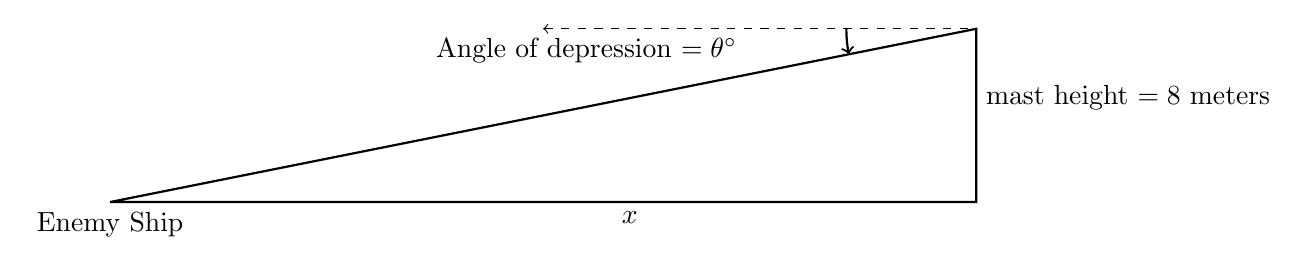
\begin{tikzpicture}[scale=1.1]
        \draw [thick] (10,0)--(0,0)--(10,2.0)--cycle;
        \draw [dashed, <-] (5,2)--(10,2.0);
        \draw [thick, ->] (8.5,2) arc [start angle=180, end angle=191.3, radius=1.5];
        \node at (5.5,2)[below]{Angle of depression $ =\theta^\circ$};
        \node at (10,1.2)[right]{mast height $=8$ meters};
        \node at (6,0)[below]{$x$};
        \node at (0,0)[below]{Enemy Ship};
      \end{tikzpicture}
    \end{center} \vspace{2cm}
    
    \item A snowman is standing 10 meters away from the base of a set of monkey bars, looking up at a boy 3 meters off the ground. The snowman is 1 meter tall.

    (a) Mark the triangle.
    
    (b) Find the angle from the snowman's head to the boy, $\theta$, to the nearest tenth degree.
    
     \hfill (not drawn to scale)
      \begin{flushright}
        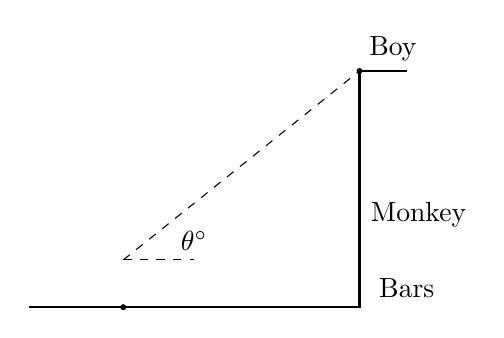
\begin{tikzpicture}[scale=0.3]
          \draw [-, dashed] (0,2)--(3,2);
          \draw [-, thick] (-4,0)--
          (0,0)--
            (10,0)--(10,10)--(12,10);
          \draw [fill] (0,0) circle [radius=0.1] node[above]{};
          \draw [fill] (10,10) circle [radius=0.1] node[above right]{Boy};
          \draw [dashed] (0,2)--(10,10);
          \node at (3, 2)[above]{$ \theta^\circ$};
          \node at (12, 0)[above]{Bars};
          \node at (12.5, 3)[above]{Monkey};
        \end{tikzpicture}
        \end{flushright}
        

\end{enumerate}
\end{document}
